%this file is drba_gb.tex
\section{Mathematical Background}
\label{sec:background}

In this chapter a mathematical basis is systematically approached to give the reader an understanding to Groebner Bases and obtaining by the Flipping-Algorithm which is needed later.\\
In the first section monomials are revisited.
The second section explains how monomials can be mathematically ordered.
After that Ideals are defined over polynomial rings and a summary on Groebner bases and Groebner fans for ideals is presented.

\subsection{Monomials}
\label{subseb:Monomials}
\newtheorem{env_definition}{Definition}[section]

First of all, the basic components of a polynomial ring has to be explained. This forms the basis of

\begin{env_definition}[Monomial] 

A \emph{monomial m} is a product of variables over a finite field $\mathbb{K}$, denoted by $ \mathbb{K} \left[X_{1},X_{2},\cdots X_{n}\right]  $ of the form $X_{1}^{u_{1}}X_{2}^{u_{2}}\cdots X_{n}^{u_{n}}$, where $u_{i}, 1 < i < n $ and $u \in \mathbb{N}_{0} $

The total \textbf{degree} of a monomial is $deg(m) = \sum_{i=1}^n u_i $ 
\end{env_definition}

\begin{env_definition}[Polynomial]

A polynomial f is a finite linear combination with coefficients $c_{u} \in \mathbb{K}$ multiplied with monomials.

\[  f = \sum_{u} c_{u}X^{u}\]\\

If $c_{u}\neq0$ then $c_{u}x_{u}$ is a term of $f$


\end{env_definition}


\subsection{Monomial Order}
\label{subsec:Monomialorder}


It is necessary to arrange the terms of a polynomial in order to compare every pair of polynomials. That is important for dividing polynomials in the finite field
$ \mathbb{K} \left[X_{1},X_{2},\cdots X_{n}\right]  $

\begin{env_definition}[Term Ordering] 

A monomial order is a relation $>$ on the set of all monomials in $\mathbb{K}\left[x\right] $ such that $\left[ 2\right] $ holds.
Let $m_{1}$,$m_{2}$ and $m_{3}$ be monomials
\begin{center}

\begin{itemize}

\item
for any pair of monomials $m_{1}$,$m_{2}$ either $m_{1} > m_{2}$ or $m_{2} > m_{1}$ or $m_{1} = m_{2}$ 
\item
if $m_{1} > m_{2} $ and $m_{2} > m_{3}$ then $m_{1} > m_{3}$
\item
$m_{1} > 1$ for any monomial $m_{1} \neq 1$
\item
if $m_{1} > m_{2}$ then $mm_{1} > mm_{2}$ for any monomial m

\end{itemize}
 
\end{center}

\end{env_definition}


Two commonly used term orders are the following.
Let $u$ and $v$ be elements of $\mathbb{N}^{n}_{0}$, such that $\left[ 2\right] $

\textbf{Lexicographic Order}
$u >_{lex} v $ if in $u-v$ the left most non-zero entry is positive.
This can be written as $X^{u} >_{lex} X^{v}$ if $u >_{lex} v $.\\


\textbf{Graded Lex Order}
$u >_{grlex} v $ if $ deg(u)>deg(v)$ or if $ deg(u)=deg(v)$ and $u >_{lex} v$

\textbf{Example} Let $m_{1} = 4x^{2}y^{4}z^{3}$ and $m_{2}= x^{1}y^{1}z^{4} \in \mathbb{K}\left[ x,y,z\right]  $.
The monomials can also be written as $m_{1} = X^{(2 \; 4 \; 3)}$ and $m_{2} = X^{(1 \; 1 \; 4)}$.
Thus $m_{1}>_{lex} m_{2}$ because the left most non-zero entry of $ (2 \; 4 \; 3) - (1 \; 1 \; 4)$ is positive.\\

The total degree of $m_{1}$ is 9 and $deg(m_{2})=6$. Hence, $m_{1}>_{lex} m_{2}$ and
$deg(m_{1})>deg(m_{2})$ so that $m_{1}>_{grlex} m_{2}$   

\textbf{Weight vectors} \\
In order to compare monomials with a generic vector $\left({a}_{1},\dots ,{a}_{n}\right)~\in \mathbb{R}^{n}_{\geq 0}$, the dot product has to be build. The highest result has the highest order. If a tie occurs, some other fixed monomial order has to be used. Note that the standard monomial orders can be expressed as weight vector. The lexicographic order needs for instance all canonical unit vectors.

\textbf{Leading term}

Given a term order $>$, each non-zero polynomial $f \in \mathbb{K}\left[ x\right] $ has a unique leading term, denoted by $lt(f)$, given by the largest involved term with respect to the term order.\\
If $lt(f) = cX^{u}$, where $c \in \mathbb{K}$, then c is the leading coefficient of $f$ and $X^{u}$ is the leading monomial(lm) or the initial monomial .$\left[ 2\right]$\\

\textbf{Example} Let $ f = 3x^{2}y^{5}z^{3} + x^{4} -2x^{3}y^{4} + 12^{2}z^{2}$ \\
With respect to lex order $f = \underline{x^{4}} -2x^{3}y^{4} + 3x^{2}y^{5}z^{3} + 12^{2}z^{2} $ \\
with respect to grlex order $f = \underline{3x^{2}y^{5}z^{3}} -2x^{3}y^{4} + x^{4}+ 12^{2}z^{2}$  \\
with respect to the weight vector 
The underlined terms are the leading binomials with the respect to the monomial order.


\subsection{Ideals}

\begin{env_definition}[Ideal]
An ideal I is collection of polynomials $f_{1}, \cdots , f_{s} \in \mathbb{K}\left[X_{1}, \cdots, X_{n}\right] $ and polynomials which can be built from these with multiplication with arbitrary polynomials and linear combination, such as $\left[1 \right]  $: \\
This is called an Ideal generated by $f_{1}, \cdots , f_{s}$ \\
\end{env_definition}

It satisfies: \\
\begin{center}

\begin{itemize}
\item
\[ \langle f_{1}, \cdots , f_{s} \rangle = \left\lbrace  \sum_{i=1}^s h_{i}f_{i} \mid h_{1}, \cdots , h_{s} \in \mathbb{K}\left[X_{1}, \cdots, X_{n}\right] \right\rbrace \]
\item
$0 \in I$ 
\item
If $f,g \in \langle f_{1}, \cdots , f_{s} \rangle$,then  $f+g \in \langle f_{1}, \cdots , f_{s} \rangle$ 
\item
If $f \in \langle f_{1}, \cdots , f_{s} \rangle$ and $h \in  \langle f_{1}, \cdots , f_{s} \rangle$, then $f \cdot h \in \langle f_{1}, \cdots , f_{s} \rangle$
\end{itemize}

\end{center}




\textbf{Example} Let $ I= \langle f_{1},f_{2} \rangle = \langle x^{2}+y, x+y+1 \rangle $ and $f=yx^{2}+y^{2}+x^{2}+xy+x$. Since $f= y \cdot f_{1} + x \cdot f_{2}, f\in I$ \begin{flushright}
$\blacklozenge$
\end{flushright} 



\begin{env_definition}[Binomial Ideal]
A binomial ideal $ I \in \mathbb{K}\left[X_{1}, \cdots, X_{n}\right]$ is a polynomial Ideal, generated by binomials. A binomial is a linear combination of two monomials.

\end{env_definition}

\begin{env_definition}[Initial Ideal]
$[TiGERS]$

\end{env_definition}

\subsection{Division Algorithm}

The reader already may determine if a polynomial $p$ lies in an Ideal $I$ in polynomial ring with one variable. This can be achieved with the help of the polynomial division.
If result has no remainder, $p$ lies in $I$
But in a ring with several variables like $ \mathbb{K} \left[X_{1},X_{2},\cdots X_{n}\right] $ the usual division algorithm can not work. A generalized algorithm is needed.\
The main goal now is to divide $g \in \mathbb{K}\left[X_{1}, \cdots, X_{n}\right] $ by 
$f_{1}, \ldots, f_{s} \in \mathbb{K}\left[X_{1}, \cdots, X_{n}\right]$, so g can be expressed in the form \begin{center}
$g = a_{1}f_{1}+ \ldots + a_{s}f_{s} +r$
\end{center} 
where the $a_{1}f_{1}+ \ldots + a_{s}f_{s} $ and $r \in \mathbb{K}\left[X_{1}, \cdots, X_{n}\right]$ \
This is possible with the Theorem mentioned at  $\left[ 3\right] $


\begin{theorem}[Division Algorithm in   ]
Fix a monomial > on $ \mathbb{Z}_{\geq 0}^{n}$ and let $ F = \left( f_{1}, \ldots, f_{s}\right) $ be an ordered s-tuple of polynomials in $ \mathbb{K}\left[X_{1}, \cdots, X_{n}\right]$. Then every  $ f \in \mathbb{K}\left[X_{1}, \cdots, X_{n}\right]$ can be written as
\begin{center}
$ f = a_{1}f_{1}+ \ldots + a_{s}f_{s} + r$
\end{center}
where $a_{i}, r \in \mathbb{K}\left[X_{1}, \cdots, X_{n}\right] $, and either $ r=0$ or r is a linear combination, with the coefficients in $\mathbb{K}$, none of which is divisible by any of
$\textsc{LT}\left(f_{1} \right), \ldots, \textsc{LT}\left(f_{s} \right)  $.
The remainder of f on division by F is r. Furthermore, if $a_{i}f_{i} \neq 0 $, then
$deg(f) \geq deg(a_{i}f_{i})$

\end{theorem}


\begin{algorithm}
\caption{Division Algorithm}\label{divisionalg}
\begin{algorithmic}[1]

\Require Basis $f_{1}, \cdots, f_{m}$ nonzero polynomials  
\Ensure $r=0$ or none of the terms in $r$ are divisible by $ LT_{\leq}\left( f_{1}\right) , \cdots , LT_{\leq} \left( f_{m}\right) $

\State $ h_{1} \gets 0 , \cdots , h_{m} \gets 0  $
\State $ r \gets 0 $
\State $ s \gets f $

\While{$s \neq 0$}
\State $ i \gets 1 $
\State  division\textunderscore occured $ \gets $  false 
\While{$i\leq m$  and division\textunderscore occured = false}
\If{$LT\left( f\left[ i\right] \right)$ divides $LT\left( s\right)  $}

\State \[ s \gets s -  \frac{LT \left( s\right)}{LT \left( f \left[ i\right] \right)}  \ast f_{i} \]
\State $h_{i} \gets h_{i} + LT\left( s\right) / LT\left( f_{i}\right) $
\State division\textunderscore occured = false
\Else
\State $i \gets i+1$
\EndIf
\EndWhile

\If{division\textunderscore occured = false}
\State $ r \gets r + \textsc{LT}\left( s\right) $
\State $ S \gets s - \textsc{LT}\left( s\right) $
\EndIf

\EndWhile


%\EndProcedure
\end{algorithmic}
\end{algorithm}


\textbf{Example}

%% TODO : Normale divsionsalgorithmus
\textbf{Example}

%% TODO : Übernehme Example 5 aus Seite 67 aus Cox, O'Shea

The last example shows that is still possible to obtain a nonzero remainder even if $f \in \langle f_{1},f_{2} \rangle $. That means r = 0 is a  necessary condition for the ideal membership but not a sufficient condition
\subsection{Groebner basis}

To solve the idea membership problem a "good" generating set for an Ideal I is needed. It would be helpful when the remainder r on division is uniqueley determined and the condition $ r = $ is equivalent to the membership in the ideal.
So the definition from $\left[KHZ \right]  $ might be useful.

\subsubsection{Definition of a Groebner basis}

\begin{env_definition}[Groebner base]
Let $\leq$ be a monomial order on $\mathbb{K}\left[X_{1}, \cdots, X_{n}\right]$ and let I be an Ideal on $ \mathbb{K}\left[X_{1}, \cdots, X_{n}\right]  $. A Groebner basis for I (with respect to $\leq$) is a finite set of polynomials $ F = \left\lbrace f_{1}, \ldots , f_{m} \right\rbrace $ in I with the property that for every nonzero $ f \in I , \textsc{LT}_{\geq}\left( f\right\rbrace $ is divisible by $\textsc{LT}\left( f_{i}\right) $ for some $ 1 \leq i \leq m $

\end{env_definition}

A Groebner basis has the beneficial property that the remainder r of f by the elements of a Groebner basis are uniquely determined and independent of the order of the elements in G.
Also every Ideal in $\mathbb{K}\left[X_{1}, \cdots, X_{n}\right]$ has a Groebner basis with respect to any monomial order $\left[ KHZ\right] $

\subsubsection{Computation of a Groebner basis}

In order to obtain a Groebner basis of an arbitrary basis $f_{1}, \ldots , f_{n}$ with an arbitrary monomial order $\geq$ of an Ideal $I$, an algorithm is needed. This algorithm is called Buchberger-Algorithm. The main idea is to build every possible S-Polynomial of $\left( f_{i},f_{j}\right) $ for every $ 1 \leq i \neq j \leq n $ and every nonzero result is added to the basis until every S-Pair of $\left( f_{i},f_{j}\right) $ vanishes.

Let the polynomials $f,g \in \mathbb{K}\left[X_{1}, \cdots, X_{n}\right] $ and $\textsc{LT}_{\leq}\left(f \right) = cX^{\upalpha} $, $\textsc{LT}_{\leq}\left(g \right) = dX^{\upbeta} $ and $\textsc{LCM}\left( X^{\upalpha},X^{\upbeta}\right) $ be the least common multiple between $X^{\upalpha}$ and $X^{\upbeta}$. 

\begin{env_definition}[S-Polynomial]
$\left[ KHZ\right] $ The S-polynomial of f and g is the polynomial
\begin{center}
\[ S\left( f,g\right) = \frac{\textsc{LCM}\left( X^{\upalpha}, X^{\upbeta}\right) }{\textsc{LT}_{\leq}\left( f\right) } \cdot f - \frac{ \textsc{LCM}\left( X^{\upalpha}, X^{\upbeta}\right) }{\textsc{LT}_{\leq}\left( g\right) } 
\cdot g \]
\end{center}

\end{env_definition}

\textbf{example} Consider the polynomials the polynomial ring $\mathbb{K}\left[ x,y,z\right] $ with
the basis $\left\lbrace f,g\right\rbrace = \left\lbrace xy^{2}-xz+y,xy-z^{2} \right\rbrace $ with respect to the lexicographic order.\\
Forming the S-Polynomial leads to:
\begin{center}
\[
 S\left( f,g\right) = \frac{\textsf{LCM}\left( xy^{2}, xy \right) } {xy^{2} } \cdot \left(  xy^{2}-xz+y\right) - \frac{\textrm{LCM}\left( xy^{2}, xy \right) } {xy } \cdot \left( xy-z \right)   
 \]  \\
 \[ = \frac{xy^{2}}{xy^{2}} \cdot \left( xy^{2}-xz+y\right) - \frac{xy^{2}}{xy} \cdot \left( xy-z\right)   \] \\
 \[ = -xz-yz+y  \]


\end{center}

\begin{flushright}
$\blacklozenge$
\end{flushright} 

The S-Polynomial is not zero and is not disvisible by the leading terms of $f$ or $g$. That means the Basis given in the example is not a Groebner basis. This can be deduced by the Buchbergers criterium.

\begin{env_definition}[Buchberger Criterion]
$\left[ KHZ\right] $ A finite set $G = \left\lbrace f_{1}, \cdots , f_{m} \right\rbrace$ of polynomials in $ \mathbb{K}\left[X_{1}, \cdots, X_{n}\right] $ is a Groebner basis of an Ideal 
$I = \langle f_{1}, \cdots , f_{m} \rangle $ if and only $S\left( f_{i},f_{j}\right) = 0$, $ \forall$  $1 \leq i,j \leq n, i\neq j $

\end{env_definition}

Now that the meaning of the S-Polynomial is clear the Buchberger algorithm can be defined.

\begin{algorithm}
\caption{Buchbergers Algorithm}\label{buchberger}
\begin{algorithmic}[1]
%\Procedure{Euclid}{$a,b$}\Comment{The g.c.d. of a and b}
\Require Basis $F = \left( f_{1}, \cdots, f_{m} \right)  $
\Ensure Groebner basis $G$ for $I = \langle f_{1}, \cdots, f_{m} \rangle $ with $ F \subseteq G $
\State $G \gets F$
\Repeat
\State $G'\gets G $
\For{each pair $f_{i}$ and $f_{j}$ in $G$ , $i\neq j$ }
\State $S \gets S\left( f_{i},f_{j} \right)^{G'}  $ \Comment{S-Polynomial with the basis of $G'$ }
\If{$G\neq 0$ }
\State $G \gets G \cup \left\lbrace S\right\rbrace $
\EndIf
\EndFor
\Until{$G = G'$}

%\EndProcedure
\end{algorithmic}
\end{algorithm}

This algorithm is correct and terminates.$\left[ KHZ\right]  $

\newpage

However, a Groebner basis is not unique. A arbitrary polynomial can be added to a Groebner basis and it is still a Groebner basis.
Fortunalety a each nonzero Ideal in $\mathbb{K}\left[X_{1}, \cdots, X_{n}\right]$ has a unique \textit{reduced} Groebner basis.

%% monic polynomial := Leading coefficient = 1
\begin{env_definition}[Reduced Groebner basis]
A Groebner basis  $G= \left\lbrace  f_{1}, \cdots , f_{m} \right\rbrace  $ in 
$ \mathbb{K}\left[X_{1}, \cdots, X_{n}\right] $ is reduced if the polynomials $f_{1},\cdots , f_{m} $ are monic and no term $f_{i}$ is divisible by $ \textsc{LT}_{\leq }\left( f_{j}\right)$ for any pair $i\neq j$, where $\leq$ is monomial order.
\end{env_definition}


\subsection{Groebner fans}
 Groebner bases for a fixed Ideal $I$ with different monomial orders can look very different and have different properties. The difference can be in the number of elements in the Groebner basis, the length or the degree of the elements. So it will be helpful if all 
possible Groebner basis of a fixed ideal can be collected together.\\
$\left[ Cox,O'Shea\right]  $ shows that the collection is finite.
 
\begin{env_definition}[Groebner fan]
$\left[ Cox,O'Shea\right]  $ A Groebner fan of an Ideal $I$ constist of finitley many closed convex polyedral cones with vertices at the origin, such that

\begin{itemize}
\item
A face of a cone $\sigma$ is $\sigma \cap \lbrace l=0\rbrace$, where $l=0$ is a nontrivial linear equation such that $l \geq 0$ on $\sigma$.
Any face of a cone in the fan is also in the fan.
\item
The intersection of two cones in the fan is a face of each.
\end{itemize}

\end{env_definition}

In order to construct a Groebner fan to a given Ideal, consider the marked Groebner basis $G = \lbrace g_{1},\cdots,g_{t}\rbrace $ of the Ideal $I$.
A marked Groebner basis is a Groebner basis where each $g \in G$ has an identified leading term, such that G is a monic Groebner basis with respect to some monomial $>$ order selecting those terms.
More informally, where all leading terms in G are marked.\\
The elements of G $g_{i}$ can be written as
\begin{center}
\[ g_{i} = x^{\upalpha\left( i\right) } +  \sum_{\upbeta} c_{i,\upbeta}x^{\upbeta}, \] 
\end{center}
where $ x^{\upalpha\left( i\right) }$ is the leading term and $ x^{\upalpha\left( i\right) } > x^{\upbeta} $,with respect to a monomial order, whenever $c_{i,\upbeta} \neq 0 $.

Now if a weight vector $\textbf{w}$ fullfills the inequation
$\upalpha\left( i\right) \ast \textbf{w} \geq \upbeta~\ast\textbf{w}$, the vector selects the correct leading term in $g_{i}$ as the term with the highest weight.\\

So the cone of a Groebner basis can be written as $ \left[Cox Oshea \right] $\\
\begin{center}
$C_{G} = \left\lbrace \textbf{w} \in \left(\mathbb{R}^{n}\right)^{+} : \upalpha\left( i\right) \cdot \textbf{w} \geq \beta \cdot \textbf{w}~~~ \textrm{whenever}~ c_{i,\upbeta} \neq 0 \right\rbrace   $
\end{center}

%% TODO: Eigenes Beispiel konstruieren??

\textbf{example}
Consider the Ideal from $\left[ Cox O'Shea\right] $ with $ I = \langle x^{2}-y,xz-y^{2}+yz \rangle \in \mathbb{Q}\left[ x,y,z\right] .$
Note that the ring is 3-dimensional so that Groebner fan can be plotted in the positive orthant $ \mathbb{R}^{3}_{+}$. \\
The marked Groebner basis with respect to the \textit{grevlex} order with $y>z>x$ is
\begin{center}
$G^{\left( 1\right) } = \left\lbrace \underline{x^{2}}-y,\underline{y^{2}} -yz -xz\right\rbrace $
\end{center}
The leading terms are underlined. Let $\textbf{w} = \left( a,b,c\right) \in \mathbb{R}^{3}_{+} $. Then W is in the cone $C_{G^{1}}$ if and only the inequalities defined above are satisfied.

\begin{itemize}

\item
$\left( 2,0,0\right) \cdot \left( a,b,c\right) \geq \left( 0,1,0\right) \cdot \left( a,b,c\right) $ or $2a\geq b$ 
\item
$\left( 0,2,0\right) \cdot \left( a,b,c\right) \geq \left( 1,0,1\right) \cdot \left( a,b,c\right) $ or $2b\geq a+c$ 
\item
$\left( 0,2,0\right) \cdot \left( a,b,c\right) \geq \left( 0,1,1\right) \cdot \left( a,b,c\right) $ or $2b\geq b+c$
\end{itemize} 

This is the first cone of the Groebner fan and can be drawn in the positive orthant sliced of the plane of $a+b+c=1$ for visuality.


%%TODO: Groebnercone hochladen


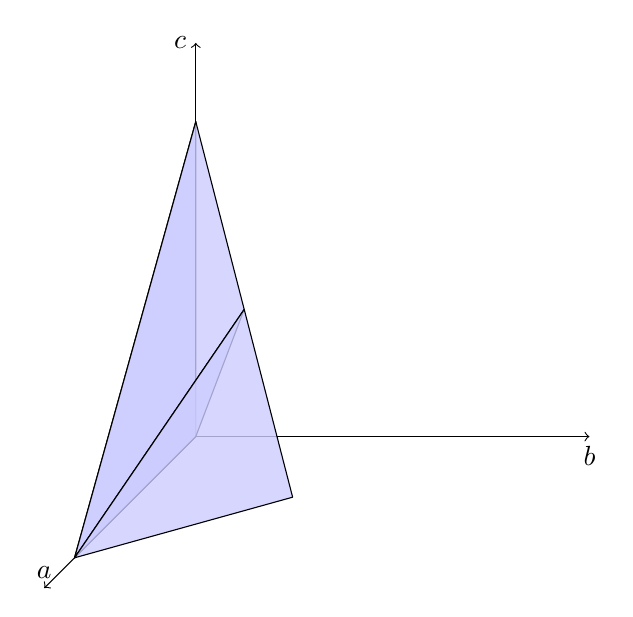
\begin{tikzpicture}[join=round]
    \tikzstyle{conefill} = [fill=blue!20,fill opacity=0.8]
    \tikzstyle{ann} = [fill=white,font=\footnotesize,inner sep=1pt]
    \tikzstyle{ghostfill} = [fill=white]
    \tikzstyle{ghostdraw} = [draw=black!50]
    
    \draw[arrows=->,line width=.4pt](0,0,0)--(0,0,5); %Z_achse
    \draw[arrows=->,line width=.4pt](0,0,0)--(0,5,0); %Y-ACHSE
    \draw[arrows=->,line width=.4pt](0,0,0)--(5,0,0); %X-ACHSE
    %\draw[arrows=<-,line width=.4pt](.42,-.767)--(4,-2);
    
    \path (5,0,0) node[below] {$b$} (0,0,5) node[above] {$a$} (0,5,0) node[left] {$c$};
    
% letzte Koordinate ist A!!!
% zweite Koordinate ist C!!!
% dritte Koordinate ist B!!!
  
 % \filldraw[conefill](0,0,0)--(4,0,0)--(2,2,0) --(1,1,2)--cycle;
 % \filldraw[conefill](0,0,0)--(0,4,0)--(2,2,0) --(1,1,2)--cycle;
%  \filldraw[conefill](0,0,0)--(1,1,2)--(4,0,0) --(0,0,4)--cycle;
%  \filldraw[conefill](0,0,0)--(1,1,2)--(0,4,0) --(0,0,4)--cycle;
\filldraw[conefill](0,0,0)--(0,4,0)--(0,0,4)--cycle;
\filldraw[conefill](0,0,0)--(0,0,4)--(1,2,1)--cycle;
\filldraw[conefill](1,2,1)--(0,4,0)--(0,0,4)--cycle;
\filldraw[conefill](1,2,1)--(0,0,4)--(2,0,2)--cycle;
 

   
\end{tikzpicture}

% % % % % % % %
\begin{flushright}
$\blacklozenge$
\end{flushright} 

This figure shows that the Groebner fan is not complete, since the cone does not cover the whole positive orthant. In this example, the other reduced Groebner basis can be obtained by applying the Buchberger Algorithm with common term orders to the Ideal $I$.
If the computed cones still are not the the whole positive orthant, then a further computation with weight vectors are necessary.

This is strategy is reasonable for a small example like above.
In genearal, the whole Groebner fan can be computed with the Groebner walk.
See $\left[ Cox OShea \right]$ for further details.\\
An inexpensive way to obtain all reduced Groebner bases of a special ideal, the Code Ideal, which will be explained later.

\subsection{Toric Ideals}
This work and is focused on Code Ideals, so it is useful to define the Toric Ideals first. Given a matrix $A =\left[a_{1},\dots, a_{n}  \right] \in \mathbb{Z}^{d \times n } $ and $u \in \mathbb{Z}^{n}$. $u$ which can be decomposed in $u^{+} $ and $u^{-}$, where $u^{+} $ and $u^{-}$ have nonnegative coefficients and disjoint support.

\begin{env_definition}[Toric Ideal]
$\left[ \textrm{Dueck Journal} \right] $ A toric ideal $I_{A}$ is defined as
\begin{center}
$ \textbf{I}_{A} = \langle \textbf{x}^{u^{+}} - \textbf{x}^{u^{-}} \mid u \in ker \left(  A \right) \rangle  $
\end{center}


\end{env_definition}

The toric ideal can also be expressed as
\begin{center}
$ \textbf{I}_{A} =  \langle \textbf{x}^{u} - \textbf{x}^{u} \mid Au = Av, u,v \in \mathbb{N}^{n}_{0} \rangle .$
\end{center}

%% TODO : Example 


\subsection{Enumerating Groebner fans}

In this section, 2 algorithms will be explained in order to enumerate the Groebner fan.
For the purpose to compute all Groebner bases from a toric ideal $I_A$ , it is necessary to search the \textit{edge graph} of a Groebner fan.\\
Two reduced Groebner bases with respect to a term order covered by the generic weight vectors $c_{1}$,$c_{2}$ are said to be adjacent if the two Groebner cones share a common \textit{facet}.

\begin{env_definition}[Facet Binomial]
$\left[TiGERS \right]  $ 
The binomial $x^{\upalpha_{k}}-x^{\upbeta_k} \in \mathcal{G}_c is a facet binomial of \mathcal{G}_c~$ if and only if there exists a $u \in \mathbb{R}^{n}$ which satisfies :
\begin{center}
\begin{enumerate}

\end{enumerate}
\item
\[ \lbrace \upalpha_{i} \cdot u > \upbeta_{i} \cdot u : i = 1, \cdots , t, i \neq k \rbrace  
\]
\item
\[ \lbrace \upbeta_{k} \cdot u > \upalpha_{k} \cdot u \rbrace \]

\end{center} 

\end{env_definition}

In the example (with the Gröebner fan) the facet binomials of a Gröbner cone determine the border to an other Gröber cone.
In order to traverse from a Gröber base $\mathcal{G}_c$ to a neighboured Gröbner base $\mathcal{G}_{c'}$ with the certain facet $x^{\upalpha}-x^{\upbeta} $, a procedure making a local change from $\mathcal{G}_c$ to $\mathcal{G}_{c'}$ is required.
This procedure is called flip.

\newpage


%TODO: Mit Input und Output ersetzten!!

\begin{algorithm}
\caption{Local change of reduced Gröbner bases in $I_A$ $\left[ TiGERS\right]  $}
\label{flip-alg}
\begin{algorithmic}[1]

\Require
Reduced Gröbner basis $ \mathcal{G} = \lbrace \underline{x}^{a}_{k}  \rbrace $ of $I_A$

A prescribed facet binomial $ \underline{x}^{a}_{i} - x^{b}_{i} \in \mathcal{G} $
\Comment {The weight vector inducing $\mathcal{G}$ is generic and the leading terms are underlined}
\Ensure The reduced Gröbner basis is adjacent to $\mathcal{G}$ in which $ \underline{x}^{b}_{i} - x^{a}_{i} $ is a facet binomial.
\State Old 
$:= \lbrace \underline{x}^{a}_{i} - x^{b}_{i} \rbrace \cup
 \lbrace \underline{x}^{a}_{j} : \underline{x}^{a}_{j} - x^{b}_{j} \in \mathcal{G},
 j \neq i \rbrace $ \Comment{Prescribed Facet and leading terms only in Old }
 \State Temp $:= \lbrace \underline{x}^{b}_{i} - x^{a}_{i} \rbrace \cup 
 \lbrace \underline{x}^{a}_{j} : x^{a}_{j} \in Old  \rbrace $
 \Comment{"Flipping" the facet Binomial}
 \State New := Computed reduced Gröbner basis with respect to the new marking 
 \Comment{This can be done with Buchberger Algorithm.}
 \State $\mathcal{G}' = \left\lbrace \underline{x}^{b}_{i} - x^{a}_{i} \right\rbrace  $
 
 \For{\textbf{each} monmial h in New}
 \State Reduce $h$ with $\mathcal{G}$ to obtain the monomial $h'$.
 \State Add $h-h'$ to $\mathcal{G}'$ with $h$ marked as the leading term.
 \EndFor
 \State Auto-reduce $\mathcal{G}'$ to get $\mathcal{G}_{new}$
 \Comment{no term shall be divisible by a leading term}

%\EndProcedure
\end{algorithmic}
\end{algorithm}

This algorithm is correct and can terminate. $ \left[ Tigers \right] $
The main advantage of the algorithm is that no weight vectors must be stored or computed.
Weight vectors are carried implicitly and that is possible due to the binomial structure that this subroutine generates for every Gröbner basis.

%% TODO Beispiel GEBEN!!!
\textbf{example}


\newpage

\subsubsection{Breadth first search}

In this section an algorithm to enumerate the edge graph of a Groebner fan via breath-first search and its drawbacks are presented.

\begin{algorithm}
\caption{Enumerating the edge graph of the Gröbner fan via breath-first search $\left[ TiGERS\right]  $}
\label{breadth-alg}
\begin{algorithmic}[1]

\Require
Any reduced Gröbner basis $ \mathcal{G}_0 $ of $I_A$
\Ensure All reduced Gröbner bases of $I_A$, (all vertices of the edge graph)
\State Todo := $\left[ \mathcal{G}_0 \right]  $
\State Verts := $\left[ \right] $
\While{Todo $\neq \emptyset$ }
\State $\mathcal{G}$ := first element in (Todo)
\State Remove $\mathcal{G} $ from Todo
\State add $\mathcal{G}$ to Verts 
\State determine list L of facet binomials of $\mathcal{G} $
\Comment{With linear programming}
 \For{\textbf{each} $x^{\upalpha}-x^{\upbeta} \in ~$ L  }
 \State $\mathcal{G}' =~$ flip($\mathcal{G},x^{\upalpha} - x^{\upbeta} $)
 \If{$\mathcal{G}' \notin \mathrm{Todo} \cup \mathrm{Verts}  $}
 \State add $\mathcal{G}'$ to Todo
 \EndIf
 \EndFor
\EndWhile \\
\Return Verts

%\EndProcedure
\end{algorithmic}
\end{algorithm}

This algorithm is intuitive but has the drawback that every vertex of the edge graph must be stored and every vertex must be checked against all other vertices if it is a new vertex or not. 
The more vertices the edge graph has, the more expensive the calculation will be. Also the need of memory will arise if a Gröbner fan has a lot of cones.
 

\subsubsection{Reverse Search tree}
In this section, a memoryless algorithm is presented which has the benefit that it runs linear depending on the size of output. The main idea is to enumerate the edge graph with depth first reverse search. The result will be a directed subgraph of the edge graph, called reverse search tree $T_{\succ}(I_{A}) $.\\
But before that, the meaning of a mismarked polynomial must be clear.
\begin{env_definition}[Mismarked Polynomial]
$\left[Tigers \right]  $
A polynomial $f$ that has been marked with respect to the monomial order $\succ$  is mismarked with respect to the monomial order $\succ$  
\end{env_definition}


\textbf{Example}
Consider the reduced Gröbner base $\mathcal{G} = \left\lbrace x^{2}y-z,y^{2}-xz, zy-xy^{2}z \right\rbrace $ 
with a certain monomial order $\succ$, which is not the lexicograpic order.
Then, the second and last term are clearly mismarked with respect to $\succ_{lex}$.

Applying the flip-procedure $(\mathcal{G},y^{2}-xz)$ leads to the Groebner base $\mathcal{G} = \{x^{2}y-z,xz^{2}-y^{2}, zy-xy^{2}z \} $. Now only the last binomial is mismarked and using flip($\mathcal{G}$, $zy-xy^{2}z$ ) the result is the reduced Groebner basis with respect to the lexicographic order $\mathcal{G} = \{xy^{2}z -xy, xz^{2}-y^{2},xy-z \} $. Note that every monomial can not be divided by the leading terms, so all Groebner bases are reduced and no auto-reduce is necessary.
 
\begin{flushright}
$\blacklozenge$
\end{flushright} 

The \textit{reverse search tree} $T_{\succ}(I_{A}) $ with a given monomal order $ \succ $ can be defined as follows.
\begin{env_definition}[Reverse Search Tree]
$TiGERS  $ For two reduced Groebner bases $ \mathcal{G}_{i}~$ and $ \mathcal{G}_{j}~$, $[\mathcal{G}_{i},\mathcal{G}_{j} ]~$ directed from $\mathcal{G}_{i}~$ to $\mathcal{G}_{j}~$ is an edge of $T_{\succ}(I_{A}) $ if $\mathcal{G_{i}}$ is obtained from $\mathcal{G_{j}}$ by the procedure flip($\mathcal{G}_{i}$,$x^{\upalpha} - x^{\upbeta}$).
$x^{\upalpha}$ is lexicographically maximal among all facet binomials of $\mathcal{G}_{i}$, that are mismarked with respect to $\succ$.
\end{env_definition}

$[TiGERS] $ ensures that the reverse search tree is an acyclic graph with a unique sink and from any reduced Groebner basis of $\mathcal{G}_{c} $ of a toric Ideal $I_{A}$, there is a unique path to the sink $\mathcal{G}_{\succ} $.
Unlike the Groebner walk procedure, there are still no weight vectors involved, but in return every facet of the Groebner cone must be computed, which can be computionally expensive for reduced Groebner basis with many polynomials.

\begin{algorithm}
\caption{Enumerating the edge graph of the Gröbner fan via reverse search $\left[ TiGERS\right]  $}
\label{reverse-alg}
\begin{algorithmic}[1]

\Require
Any reduced Gröbner basis $ \mathcal{R}_{\succ} $ of $I_A$ and its term order $\succ$
\Ensure All reduced Gröbner bases of $I_A$, (all vertices of the edge graph)
\State $\mathcal{G} := \mathcal{R}_{\succ} $
\State $j := 0$
\State $L := $ list of facet binomials of $\mathcal{G}$ marked by $\succ$
\State add $\mathcal{G}$ to output
\Repeat
\While{ $ j < \left|L\right| $ }

\State j := j + 1
\State $\mathcal{G}':= $ flip($\mathcal{G}$,$L[j]$);

\If{ $[\mathcal{G}',\mathcal{G}] \in T_{\succ}(I_{A}) $ }
\Comment{ Check for adjacency }
\State $\mathcal{G} := \mathcal{G}' $  
\State $ j := 0$
\State $ L := $ list of facet of $\mathcal{G}$ marked by $\succ$
\State add $ \mathcal{G}$ to output

\EndIf 

\EndWhile

\If{$ \mathcal{G} \neq \mathcal{R}_{\succ}$}
\State $\mathcal{G}' :=~$ unique element such that $[\mathcal{G}',\mathcal{G}] \in T_{\succ}(I_{A}) $
\State $j := 0$
\State $L := $ list of facets of $\mathcal{G}'$ marked by $\succ$

\Repeat
\State $j := j + 1$
\Until{the common facet of $\mathcal{G}$ and $\mathcal{G}'$ is the $j$-th facet of $L$ }

\EndIf

\Until{$\mathcal{G} = \mathcal{R}_{\succ}$ and $ j = \left|L\right| $ }


%\EndProcedure
\end{algorithmic}
\end{algorithm}

\textbf{Example}
Consider the Ideal with the reduced Groebner basis with respect to the lexicographic order $x_{1} \succ \ldots \succ x_{6} $
\[ \mathcal{G} = \{x_{1} - x_{2}, x_{3} - x_{4}, x_{5}-x_{6} , x_{2}^{2} -1 , x_{4}^{2} - 1, x_{6}^{2} - 1 \} \]

Applying the breath-first search algorithm for this reduced Groebner basis results to the following edge graph.\\

%TODO: BREITENSUCHENGRAPH HOCHLADEN

Using the reverse search method, this search tree results.

%TODO: REVERSE SEARCH GRAPGH




\begin{figure}[htb]
\centering
\begin{tikzpicture}
	\draw (0,0) node[above] {$\mathcal{G}_1$}
				(-2,-2) node[below] {$\mathcal{G}_2$}
				(0,-2) node[below] {$\mathcal{G}_4$}
				(2,-2) node[below] {$\mathcal{G}_8$}
				(-2,-4.5) node[below] {$\mathcal{G}_3$}
				(0,-4.5) node[below] {$\mathcal{G}_5$}
				(2,-4.5) node[below] {$\mathcal{G}_7$}
				(0,-7) node[below] {$\mathcal{G}_6$};
    \draw [<-] (0.2,0) -- (2,-2);
	\draw [<-] (0,0) -- (0,-2);
	\draw [<-] (-0.2,0) -- (-2,-2);
	\draw [<-] (-2,-2.5) -- (-2,-4.5);
	\draw [<-] (0,-2.5) -- (0,-4.5);
	\draw [<-] (0.2,-2.5) -- (2,-4.5);
	\draw [<-] (0,-5) -- (0,-7);
\end{tikzpicture}
\caption{The reverse search tree for $\mathcal{G}_{1}$}%
\label{fig:rev}%
\end{figure}

\begin{figure}[htb]
\centering
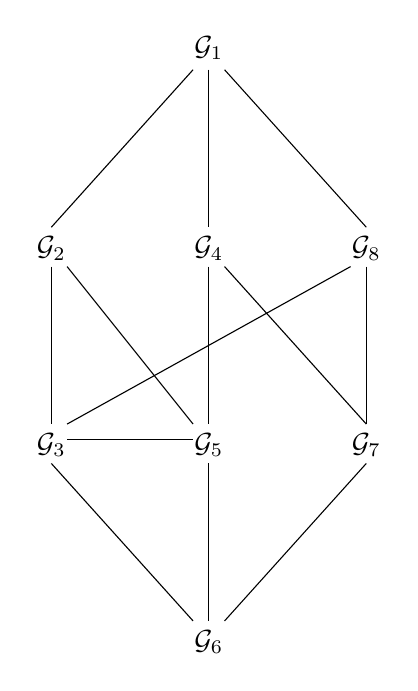
\begin{tikzpicture}
	\draw (0,0) node[above] {$\mathcal{G}_1$}
				(-2,-2) node[below] {$\mathcal{G}_2$}
				(0,-2) node[below] {$\mathcal{G}_4$}
				(2,-2) node[below] {$\mathcal{G}_8$}
				(-2,-4.5) node[below] {$\mathcal{G}_3$}
				(0,-4.5) node[below] {$\mathcal{G}_5$}
				(2,-4.5) node[below] {$\mathcal{G}_7$}
				(0,-7) node[below] {$\mathcal{G}_6$};
    \draw [-] (0.2,0) -- (2,-2); % G1 - G2
	\draw [-] (0,0) -- (0,-2);   % G1 - G4
	\draw [-] (-0.2,0) -- (-2,-2); % G1 - G8
	\draw [-] (-2,-2.5) -- (-2,-4.5); % G2 - G3
	\draw [-] (0,-2.5) -- (0,-4.5); % G4 - G5
	\draw [-] (0.2,-2.5) -- (2,-4.5); % G4 - G7
	\draw [-] (0,-5) -- (0,-7); % G5 - G6
	\draw [-] (-1.8,-4.7) -- (-0.2,-4.7); % G3 - G5
	\draw [-] (-2,-5) -- (-0.2,-7); %G3 - G6
	\draw [-] (-1.8,-2.5) -- (-0.2,-4.5); % G2 - G5
	\draw [-] (-1.8,-4.5) -- (1.8,-2.5); % G3 - G8
	\draw [-] (2,-2.5) -- (2,-4.5); % G8 - G7
	\draw [-] (0.2,-7) -- (2,-5); %G6 - G7

\end{tikzpicture}
\caption{The complete edge graph via breadth first search}%
\label{fig:breadth}%
\end{figure}

%TODO: Kanten mit den flipp binomials beschreiben und alle Groebnerbase aufschreiben



Even for this small example a lot of edges were saved.
\ref{fig:breadth}.


\subsection{Degree compatible Groebner}
Computing the whole Groebner fan can be very expensive and not every cone is interesting.
In this section, the degree compatible Groebner fan is introduced and how the algorithm can
be changed so that only the degree compatible Groebner fan will be computed.\\
\begin{env_definition}[Degree compatible Groebner basis]
$[dueck paper] $
A reduced Groebner basis for an ideal I with respect to a certain monomial order is
degree compatible if and only if the corresponding Groebner cone contains the all-one vector 1.
\end{env_definition}
Equivalent to this, the leading term must have the highest degree.

Since a Groebner fan is homogenous at $\mathbb{R}^{n}_{+}$, there will be at least one degree compatible Groebner basis.
That is a special case can be easily determined as follows.

\begin{env_definition}[Only degree compatible Groebner basis]
$[dueck paper] $
A Groebner basis $\mathcal{G}$ with respect to a degree compatible monomial ordering $\succ$  is the only degree compatible Groebner basis for an Ideal if and only if
\[ deg(x^{a}) > deg(x^{b})~~ \forall~~ x^{a}-x^{b}\in \mathcal{G} \] 
\end{env_definition}

This can be also described by the all-one vector that lies completely in a Groebner cone of a Groebner basis $\mathcal{G}$.
It follows that the all-one vector does not cut any facets if there is only one degree compatible Groebner basis. \\

The algorithms 4 and 5 can be adapted in order to compute only the degree compatible Groebner fan.\\ \\
The breadth-first search now needs a degree compatible Groebner basis as an input. This can be achieved by applying the Buchberger Algorithm with a degree compatible monomial, for example the grlex order. After that it is required that the Groebner basis is checked if its is the only degree compatible basis. %see only degree compatible Groebner basis
Also the only facet binomials x$^{a}$ - x$^{b}$ which are allow to be "flipped" are the binomials that fulfills the condition
deg(x$^{a}$ ) = deg(x$^{b} $ ). \\ \\
The reverse search tree can be deployed as in Definition 2.14 but with the restriction that deg(x$^{a}$ ) = deg(x$^{b}$) must be fulfilled to traverse the degree compatible Groebner fan.
$[dueckpaper, Lemma 2.2]$ guarantees that at least one such facet binomial will be found. 
The sink of the reverse search tree contains binomials that are not mismarked with respect to the grlex order. 

   



\subsection{Linear Codes over Prime Fields}
This work is concentrated on computing the Groebner fan of a linear code. Now the mathematic background of the Groebner fans is given, the linear Codes and Code Ideals have to be defined to give a connection between these two topics.\\ \\
Let $\mathbb{F}$ be a finite field and let $n~$ and $k~\in \mathbb{N}~$ with $n\geq k$.
\begin{env_definition}[Linear Code]
$ [Dueck Journal ] $ A linear code of length n and dimension k over $\mathbb{F}~$ is the image $\mathcal{C}~$ of a injective linear mapping $\phi~:~\mathbb{F}^{k} \rightarrow \mathbb{F}^{n}  $
\end{env_definition} 

Such a code will be denoted als an [$n$,$k$] code and its elements are called codewords. The codewords are written 
as row vectors. The Code $\mathcal{C}~$ can alternatively be described as row space matrix of $G \in \mathbb{F}^{k \times n}$. The rows of $G$ form a basis of $\mathcal{C}~$.
$G$ is also calles \textit{generator matrix} for $\mathcal{C}$.

\begin{env_definition}[Standard form]
$[dueckjournal]$
A $[n,k]~$ code $\mathcal{C}~$ is in standard form if it has a generator matrix like $G = (I_{k}| M)$, where $I_{k}$ is the $k \times k$ matrix.
\end{env_definition}


\textbf{Example}
Consider the binary $[7,4]$ Hamming Code with its generator matrix

\[
G =
\begin{pmatrix}
1 & 0 & 0 & 0 & 1 & 1 & 0 \\ 
0 & 1 & 0 & 0 & 1 & 0 & 1 \\  
0 & 0 & 1 & 0 & 1 & 1 & 1 \\ 
0 & 0 & 0 & 1 & 0 & 1 & 1
\end{pmatrix} 
\]

The code $c~$ of the word $x~$ is obtained with the vector-multiplication
\[
     xG = c \\
 \]
 Let x be $\left(1,0,1,0\right)$, then the codeword c results to:
 \[
      \left(1,0,1,0\right) \cdot \begin{pmatrix}
      1 & 0 & 0 & 0 & 1 & 1 & 0 \\ 
      0 & 1 & 0 & 0 & 1 & 0 & 1 \\  
      0 & 0 & 1 & 0 & 1 & 1 & 1 \\ 
      0 & 0 & 0 & 1 & 0 & 1 & 1
      \end{pmatrix}   = \left(1,0,1,0,0,0,1\right) \\
  \]
\begin{flushright}
$\blacklozenge$
\end{flushright} 

Two codes are equivalent if one generator matrix can be obtained from the other by permutating columns and rows.
It follows that every linear code is equivalent to a linear code in standard form.$[dueckjournal]$ \\

A linear Code $\mathcal{C}$ can be \textit{punctured} by deleting the same coordinate $i$ in each codeword.
%TODO: mehr zu punktierten Codes schreiben


\subsection{Code Ideals}
\label{subsec:codeideals}
In this section, the linear codes and the Groebner bases come together.\\
Each linear code $\mathcal{C}~$ can be associated to a binomial ideal.$[dueckpaper]$ Let $\mathcal{C}~$ be a $[n,k]$ code and let 
$\mathbb{K}[\textbf{x}]~=~\mathbb{K}[x_{1},\cdots,x_{n}]$.
Then the \textit{code ideal} can be defined as follows:

\begin{env_definition}[Code Ideal]
$[dueckpaper]$ A code ideal $I(\mathcal{C})$ is the union between the toric ideal and a nonprime ideal $I_{p}$, such that
\begin{center}
$ I_{\mathcal{C}} = \langle \textbf{x}^{c} - \textbf{x}^{c'} | c - c' \in \mathcal{C}  \rangle + I_{p},$\\
\textrm{where}
 $I_{p} = \langle x_{i}^{p} - 1 | 1 \leq i \leq n \rangle $
\end{center}
\end{env_definition}


\textbf{Example} Let $\mathcal{C}_{1}~$ be a binary $[6,3]$ code with generator matrix
\[
G_{1} =
\begin{pmatrix}
1 & 0 & 0 & 0 & 1 & 0 \\ 
0 & 1 & 0 & 1 & 1 & 1 \\  
0 & 0 & 1 & 0 & 1 & 0  
\end{pmatrix} 
\]

The associated code Ideal $I(\mathcal{C})$ leads to: \newline
\begin{center}
$I(\mathcal{C}) = \{x_{1}-x_{5},x_{2}-x_{4}x_{5}x_{6},x_{3}-x_{5}  \} \cup \{x_{1}^{2}-1,x_{2}^{2}-1,x_{3}^{2}-1,x_{4}^{2}-1,x_{5}^{2}-1,x_{6}^{2}-1\}  $
\end{center}
Note that the terms $x_{1}^{2}-1,~x_{2}^{2}-1,~x_{3}^{2}-1 $ are divisible by the leading terms of the toric ideal.
The reduced Groebner basis $\mathcal{G}_{\succ}$ with respect to the lexicographic ordering $\succ$ with $x_{1} \succ \cdots \succ x_{6}$ is:
\begin{center}
$ \mathcal{G}_{\succ} = \{x_{1}-x_{5},x_{2}-x_{4}x_{5}x_{6},x_{3}-x_{5}  \} \cup \{x_{4}^{2}-1,x_{5}^{2}-1,x_{6}^{2}-1  \}  $
\end{center}

\begin{flushright}
$\blacklozenge$
\end{flushright} 

 

\newpage
